\subsection{Przykładowe wykresy dal $\varepsilon = 10^{-4}$.}
\begin{figure}[h]
    \centering
    \begin{subfigure}{.5\textwidth}
      \centering
      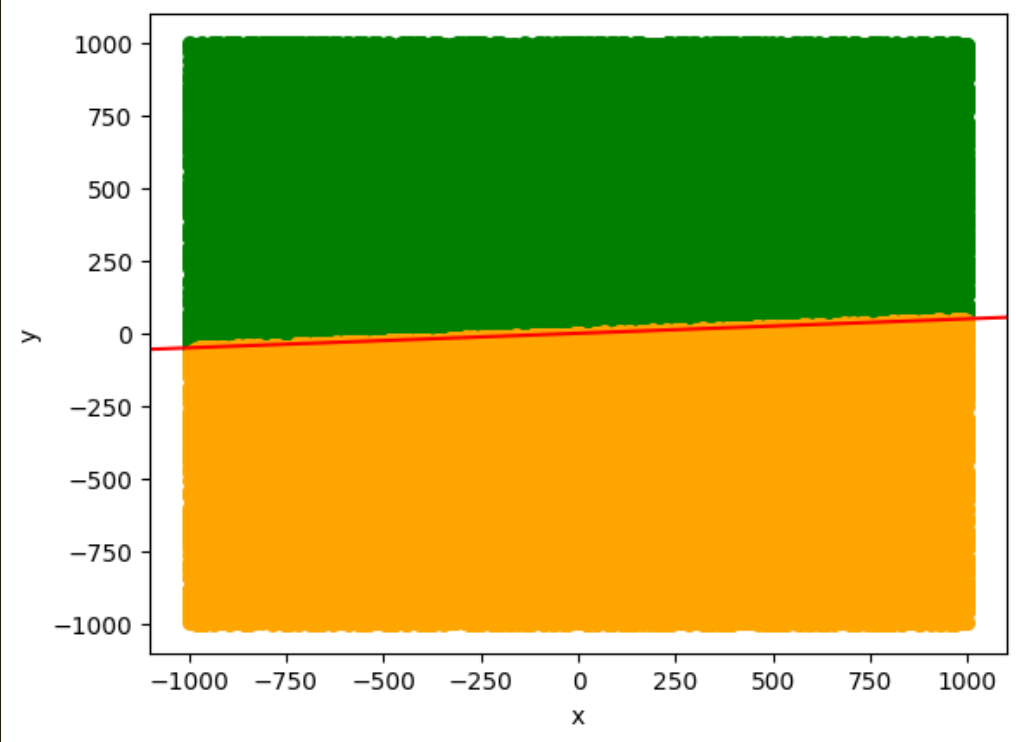
\includegraphics[width=.9\linewidth]{1k.png}
      \caption{$10^5$ losowych punktów $(x, y) \in \left[-1000,1000\right]^{2}$.}
      \label{fig:sub1}
    \end{subfigure}%
    \begin{subfigure}{.5\textwidth}
      \centering
      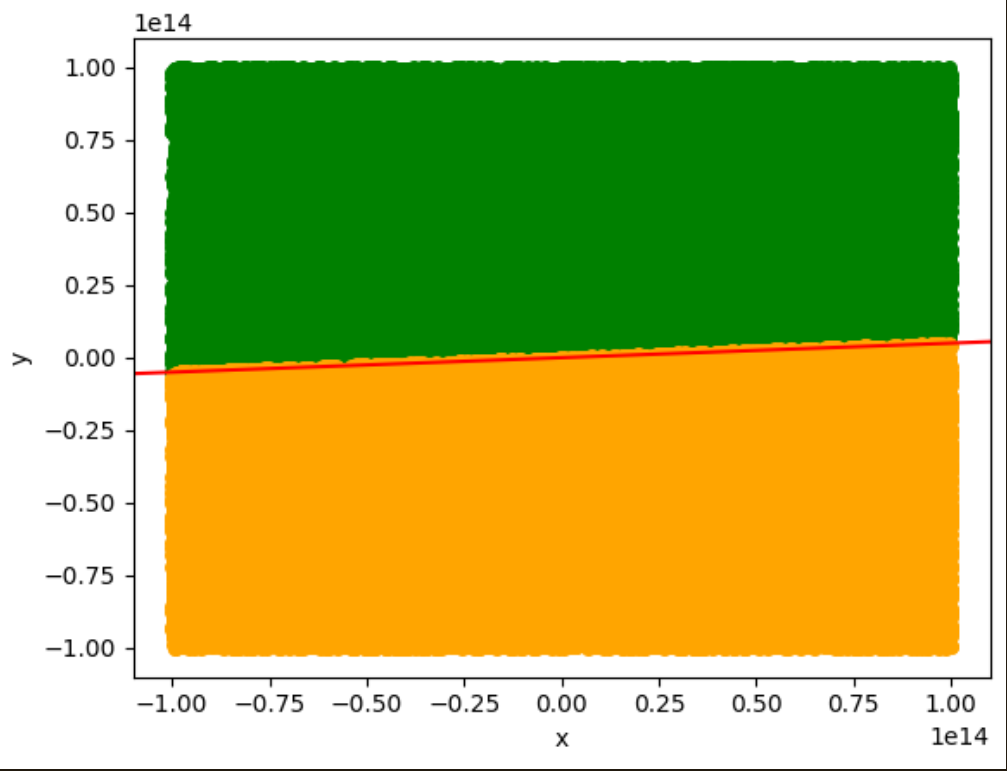
\includegraphics[width=.9\linewidth]{2k.png}
      \caption{$10^5$ losowych punktów $(x, y) \in \left[-10^{14},10^{14}\right]^{2}$.}
      \label{fig:sub2}
    \end{subfigure}
    \label{fig:test}
    \end{figure}
    
    \begin{figure}[h]
    \centering
    \begin{minipage}{.5\textwidth}
      \centering
      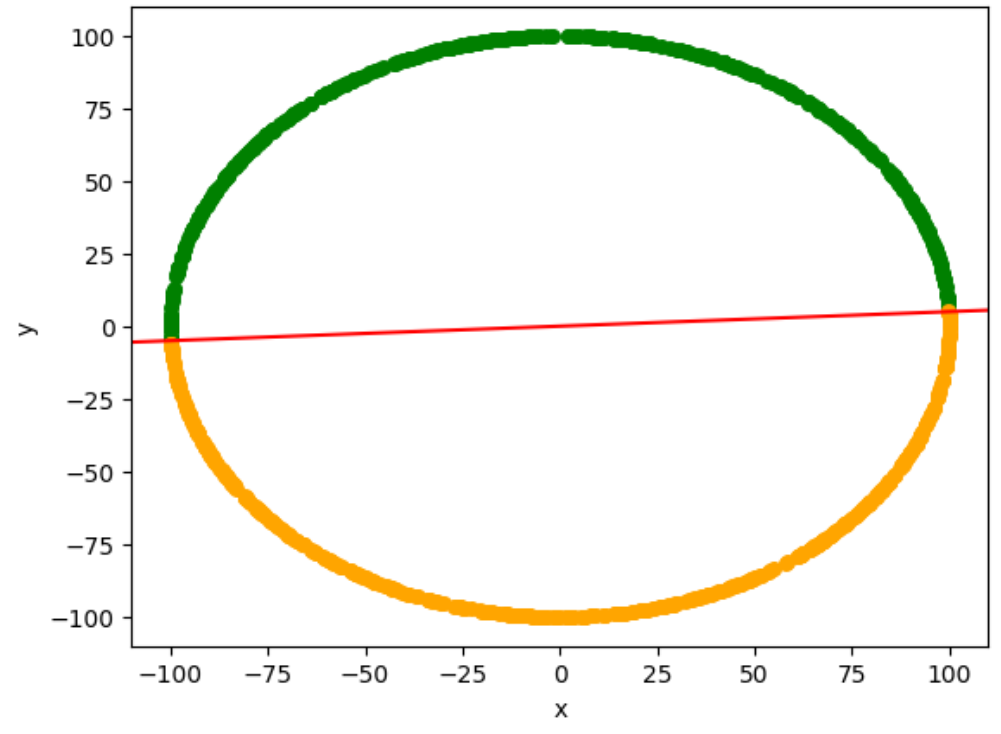
\includegraphics[width=.9\linewidth]{3k.png}
      \caption{$1000$ losowych punktów leżących na okręgu.}
      \label{fig:test1}
    \end{minipage}%
    \begin{minipage}{.5\textwidth}
      \centering
      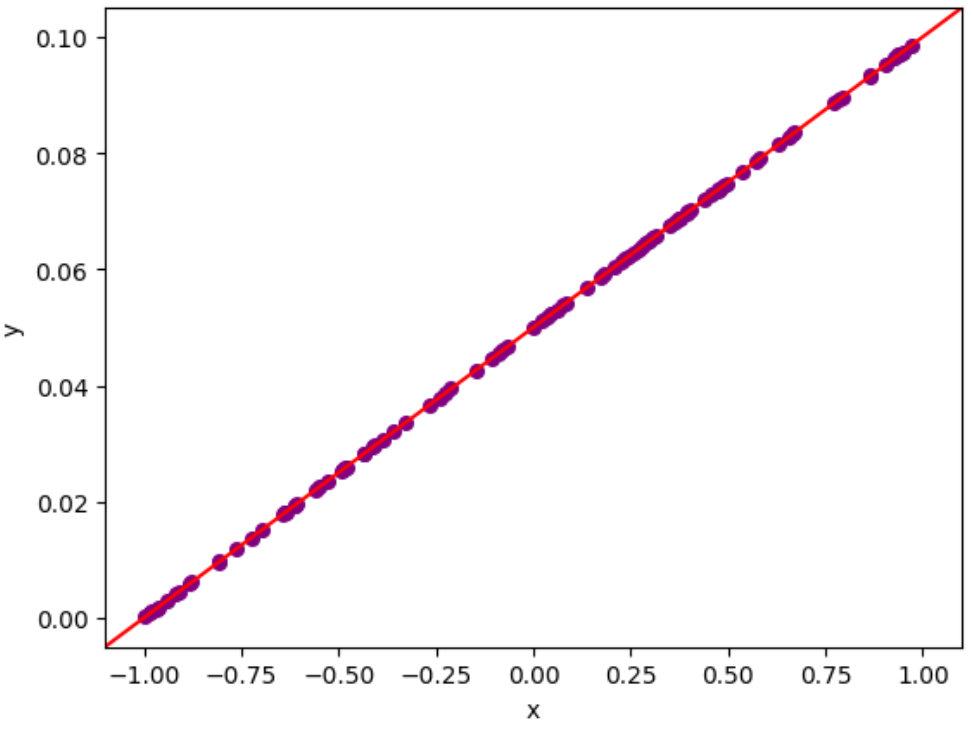
\includegraphics[width=.9\linewidth]{4k.png}
      \captionof{figure}{$ 1000$ losowych punktów na prostej.}
      \label{fig:test2}
    \end{minipage}
    \end{figure}
\subsection{Tabele}
\quad Poniżej przedstawione są tabele ilości zaklasyfikowanych punktów
 ze zbiorów \\ (a, b, c, d) ze względu na ich położenie od prostej, $\varepsilon$ tolerancje
 wartości bliskich zera oraz funkcje użytą dla obliczenia wyznacznika.\\ \\

 \begin{figure}[!hbt]
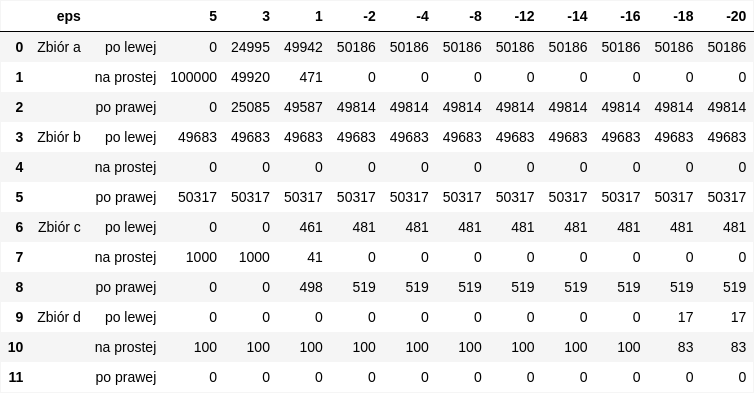
\includegraphics[scale=0.6]{eps_compar.png}
\caption*{Numpy $3\times 3$.}
 \end{figure}
 \begin{figure}[!hbt]
    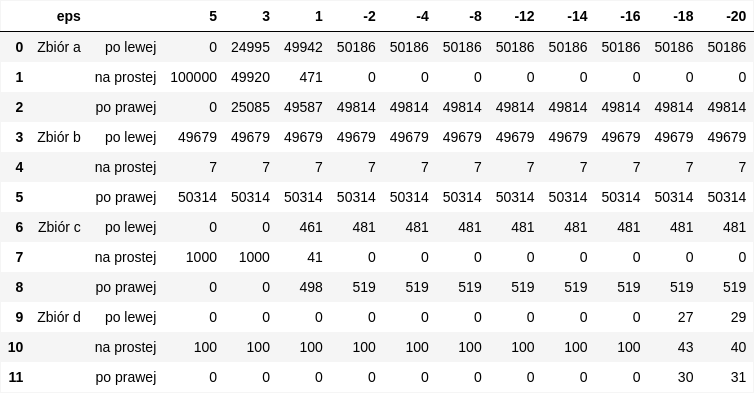
\includegraphics[scale=0.6]{eps_compar2l.png}
    \caption*{Numpy $2\times 2$.}
     \end{figure}
     \begin{figure}[!hbt]
        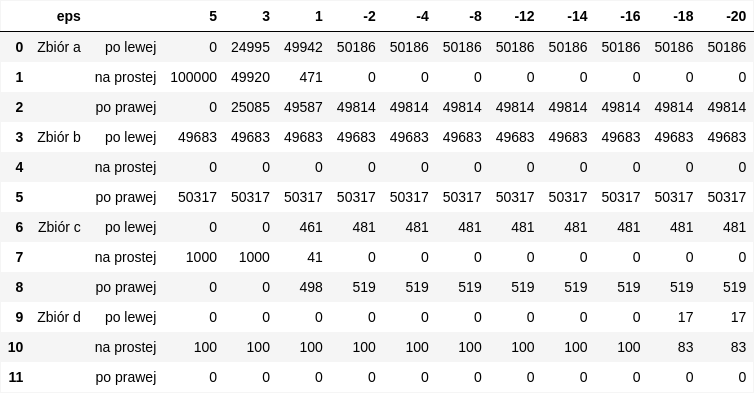
\includegraphics[scale=0.6]{eps_compar.png}
        \caption*{Własna funkcja $3\times 3$.}
        \end{figure}
         \begin{figure}[!h]
            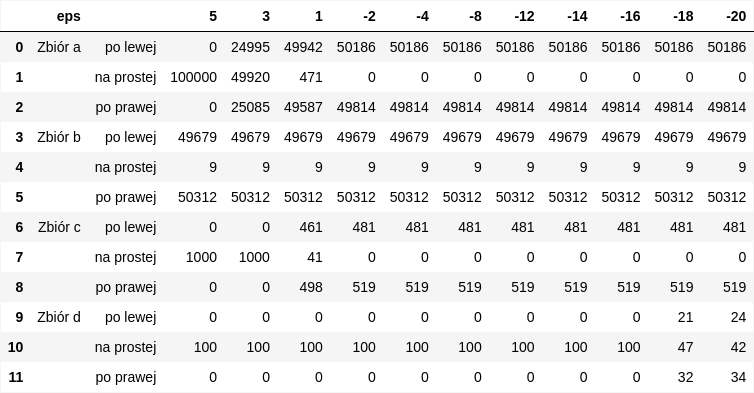
\includegraphics[scale=0.6]{eps_compar2.png}
            \caption*{Własna funkcja $2\times 2$.}
             \end{figure}
             -
             \newpage 
             \centerline{\rule{20cm}{0.4pt}}
\subsection{Analiza wyników}
\quad Na potrzeby analizy danych wybierzemy wyniki dla bibliotecznej 
funkcji liczenia wyznacznika $3 \times 3$.
\begin{enumerate}
    \item W zbiorze $a$ dla $\varepsilon \leq 10^{-2}$ widzimy brak zmian 
w ilości zaklasyfikowanych do różnych zbiorów punktów. Także charakterystyczną dla tego $\varepsilon$ 
cechą można nazwać $0$ punktów rozpoznanych jako leżące na prostej.\\
Żeby zweryfikować nasze wyniki policzmy prawdopodobieństwo, że punkt w naszym zbiorze zostanie 
wylosowany w miejscu dla którego będzie zaklasyfikowany, jako należący do prostej. 
W naszych obliczeniach dla prostoty pominiemy niepewności związane z obliczeniami komputerowymi.\\
Klasyfikujemy punkty do odpowiedniej grupy obliczając iloczyn wektorowy
$\overrightarrow{ab} \times \overrightarrow{ac}$, gdzie $ c = (x,y)$ jest punktem, dla którego poszukujemy wiadomości o lokalizacji względem prostej przechodzącej przez punkty $ a$ i $ b$. Metoda ta jest równoznaczna z obliczeniem wyznacznika macierzy $ 2\times2$:  

$$
(1)\det(a, b, c)= \begin{vmatrix}
       a_{x} - c_{x} & a_{y} - c_{y} \\
       b_{x} - c_{x} & b_{y} - c_{y} 
              \end{vmatrix}.
$$\\
Wiemy także, że iloczyn wektorowy $\overrightarrow{A} \times \overrightarrow{B}$ można także obliczyć ze wzoru: 
$$
\overrightarrow{A} \times \overrightarrow{B} = ||A|| \cdot ||B|| \cdot \sin{\theta}.
$$
Gdzie $\sin{\theta}$ to kąt pomiędzy wektorami $\overrightarrow{A}$ i $\overrightarrow{B}$.\\
Wybierzmy teraz dla konkretnego punktu $c$ takie $a$ i $b$ na prostej, żeby 
\begin{enumerate}
    \item Dla $A = \overrightarrow{ab}, ||{A}|| = 1$.
    \item $\sin{\theta} = 1$, gdzie $\theta$ jest kątem pomiędzy $\overrightarrow{ab}$ i $\overrightarrow{ac}$ (wektor $\overrightarrow{ac}$ jest prostopadły do naszej prostej i do wektora $\overrightarrow{ab}$).
\end{enumerate}
Wtedy nasz iloczyn $$\overrightarrow{A} \times \overrightarrow{B} = ||A|| \cdot ||B|| = 1 \cdot ||B|| = ||B||.$$
I pytanie klasyfikacji punktu jako należacego do prostej sprowadza się do sprawdzenia czy $||B|| < \varepsilon$.
Dla zbioru $a$ długość prostej o równaniu $y = \frac{1}{20}x - 1$ na całym zbiorze $(-1000, 1000)$ jest równa 
$$
    \sqrt{(y(1000) - y(-1000))^2 + (1000 + 1000)^2} = \sqrt{10 ^ 4 + 4 \cdot 10^6} = \sqrt{4,01 \cdot 10^6} \approx 2 \cdot 10^3.
$$
Pole obszaru na którym punkty będą klasyfikowane jako należące do prostej zate wynosi
$$
    2 \cdot 2 \cdot 10^3 \cdot \varepsilon = 4 \cdot 10^3 \cdot \varepsilon.
$$
Teraz w porównaniu do całkowitego pola naszego zbioru
$$
    \frac{4 \cdot 10^3 \cdot \varepsilon}{(1000 - (-1000))^2}=
    \frac{4 \cdot 10^3 \cdot \varepsilon}{4 \cdot 10^6} =  10^{-3} \cdot \varepsilon.
$$
Patrząc na ten wynik dla $\varepsilon = 10^{-2}$ nie jest zadziwiające to, że 
żaden z $10^5$ punktów nie został zakwalifikowany jako leżący na prostej. Gdzyż prawdopodobieństwo 
wylosowania takiego punktu to tylko $10^{-5}$.
\item Dla zbioru b widzimy, że dla wszystkich $10^{-20} < \varepsilon < 10^5$ dostajemy ten sam wynik 
, czego też warto było się spodziewać gdzyż stosując metodę opisaną w poprzednim podpunkcie dostajemy 
prawdopodobieństwo wylosowania punktu leżącego na prostej 
$$
    \frac{4 \cdot 10^{14} \cdot \varepsilon}{(10^{14} - (-10^{14}))^2}=
    \frac{4 \cdot 10^{14} \cdot \varepsilon}{4 \cdot 10^{28}} =  10^{-14} \cdot \varepsilon.
$$
Czyli nawet dla $\varepsilon = 10^5$ prawdopodobieństwo, że conajmniej z $10^5$ punktów zostanie zaklasyfikowany 
do prostej to około $10^{-4}$.
\item Dla zbioru c widzimy podobną sytuację. Dla $\varepsilon > 10^{-2}$ 
każde zmniejszenie $\varepsilon$ powoduje ogromne zmiany w wynikach, ale podalsze zwiększenie precyzji 
nie ma żadnego efektu na wynikach.

\item Dla zbioru d zmniejszenie $\varepsilon$ ma największe znaczenie ze wszystkich. 
Nawet przejście pomiędzy $\varepsilon = 10^{-16}$ do $\varepsilon = 10^{-18}$ ma ogromne znaczenie 
na ilości punktów zakwalifikowanych do prostej.
\end{enumerate}